% Very simple template for lab reports. Most common packages are already included.
\documentclass[a4paper, 11pt]{article}
\usepackage[utf8]{inputenc} % Change according your file encoding
\usepackage{graphicx}
\usepackage{parskip}
\usepackage{url}

%opening
\title{Rudy --- A small web server}
\author{Anton Bothin}
\date{\today{}}

\begin{document}

\maketitle

\section{Introduction}

The assignment was to build a small web server using Erlang. This was done by creating a HTTP parser as well as using a socket API.

The goal, besides learning Erlang, was to gain an understanding of some concepts used in creating distributed systems. These concepts consisted of using the HTTP protocol, using sockets, and creating server processes.

\section{Main problems and solutions}

The assignment consisted of two main parts: creating the HTTP parser, and creating the server using a socket API. 

The HTTP parser consisted of splitting a HTTP request into its different components. According to the RFC 2616 format this resulted in three different components: request-line, headers, and body. The code for the HTTP parser was already provided, it worked by recursively traversing the request looking for certain character combinations that marked the end of each component while consuming each character up to that point.

The HTTP server also had an almost complete codebase already provided. This implementation consisted of four procedures: init, handler, request and reply.

\begin{itemize}

\item \texttt{init(Port)} initializes a listening socket on the specified port. The socket is then passed to \texttt{handler/1} which was done by calling \texttt{handler(Listen)} where the ``:'' was marked.

\item \texttt{handler(Listen)} listens to the socket for an incoming request. When a client is connected the request should be handled by \texttt{request/1} before the connection is closed. This was done by calling \texttt{request(Client)} where the ``:'' was marked.

\item \texttt{request(Client)} reads the request and parses it using the HTTP parser. This parsing was done by adding \verb|Request = http:parse_request(Str)| where ``:'' was marked. The parsed request is after this passed to \texttt{reply/1}.

\item \texttt{reply(Request)} generates a reply based on the request using the \texttt{ok/1} procedure. In my case the argument passed to \texttt{ok/1} is simply the URI that was entered. 

\end{itemize}

One problem, which was also specified in the assignment, was that the server terminated after one request. This was solved by modifying \texttt{handler/1} to recursively call itself after a request has been handled.

\section{Evaluation}

To test the server I used the provided benchmark program. A small delay of 40ms was also added to the handling of requests to simulate file handling, server side scripting, etc. The entire test program took 4688ms to run, since the program sent 100 requests this is the same as 46.88ms/request giving us a throughput of 21.33 requests/s. From this we can see that the delay is significant since it makes up more than 85\% of the runtime.

Running the benchmark on several machines at the same time gave the following results:

\begin{figure}[!h]
  \begin{center}
    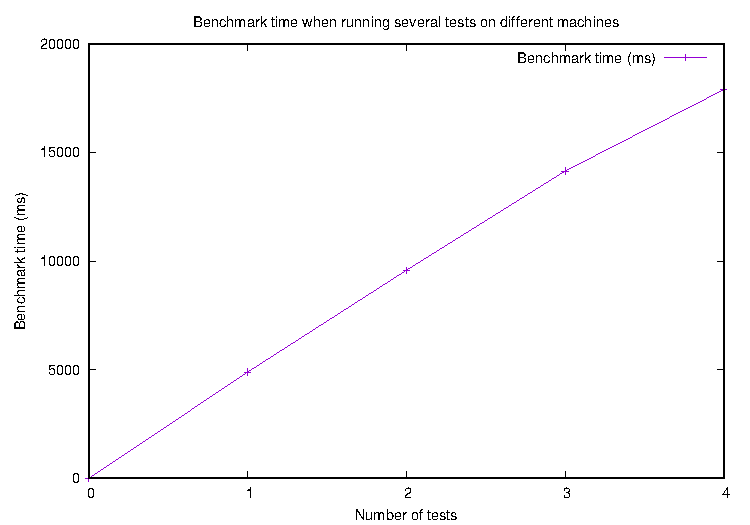
\includegraphics[width=120mm]{results1.pdf}
    \caption{Benchmark time when running several tests on different machines}
    \label{fig:results1}
  \end{center}
\end{figure}

As seen above, figure \ref{fig:results1} shows a linear pattern which is expected as the program only runs on one thread. When running the multithreaded version which was provided, the time was the same when running several benchmarks as when running just one. I could however see that the overhead became a tiny bit larger when running multiple threads, this is probably due to the fact that several processses are created.

\section{Conclusions}

This seminar was useful for learning the basics of Erlang. It also reminded me of how a HTTP request is structured as well as how a server is built.

\end{document}
